% !TeX root = ../../main.tex
% Add the above to each chapter to make compiling the PDF easier in some editors.

\section{Benchmark Procedure}\label{ord:ch4:sec5}
% 
The benchmark study is realized within a label tool, that was implemented in the scope of this thesis in the integrated development environment \textit{HDevelop} from MVTec.
Within the labeltool also the four interactive methods are implemented.
The collection of the benchmark statistics is also realized within this program.
The labeltool provides a user interface with various windows as shown in Figure \ref{fig:ch4:sec4:labeltool}.

% Introduction for each participants.
Each participant got an introduction to the labeltool, before they started.
% 'Do as long as you want'-policy
The time spent for the participation in the benchmark varied between the users, due to their available working time. % company time.
% TODO get average time spent and average annotations
The average participation time was XXX minutes and included XXX annotations.
% Random order of the images to enable an equal coverage of all images
Therefore, for each benchmark user the images were arranged randomly, in order to ensure a uniform coverage of the images.

% Label task.
The task of the participant is to create a segmentation mask for the single objects in the image.
To create a mask, one of the four interactive methods needs to be applied.
% Free choice of methods.
The user can choose which method to apply.
Thereby, statistics on the same object are obtained, that are created by various methods.
Further, the participation in the benchmark study was kept interesting, by giving the participants a free choice which method to choose.
% Label RoI.
The task to label each object was limited to the objects inside a polygon, that is referred to as label region, as illustrated in Figure \ref{fig:ch4:sec4:labeltool}.
Thereby, not all objects in an image should be labeled, in order to realize a reasonable participation time.
It is not part of the user's task to assign a class name for the created annotation.
% Label instructions
An additional label instruction was provided partially, to clarify the scope and avoid misunderstandings.

\begin{figure}
	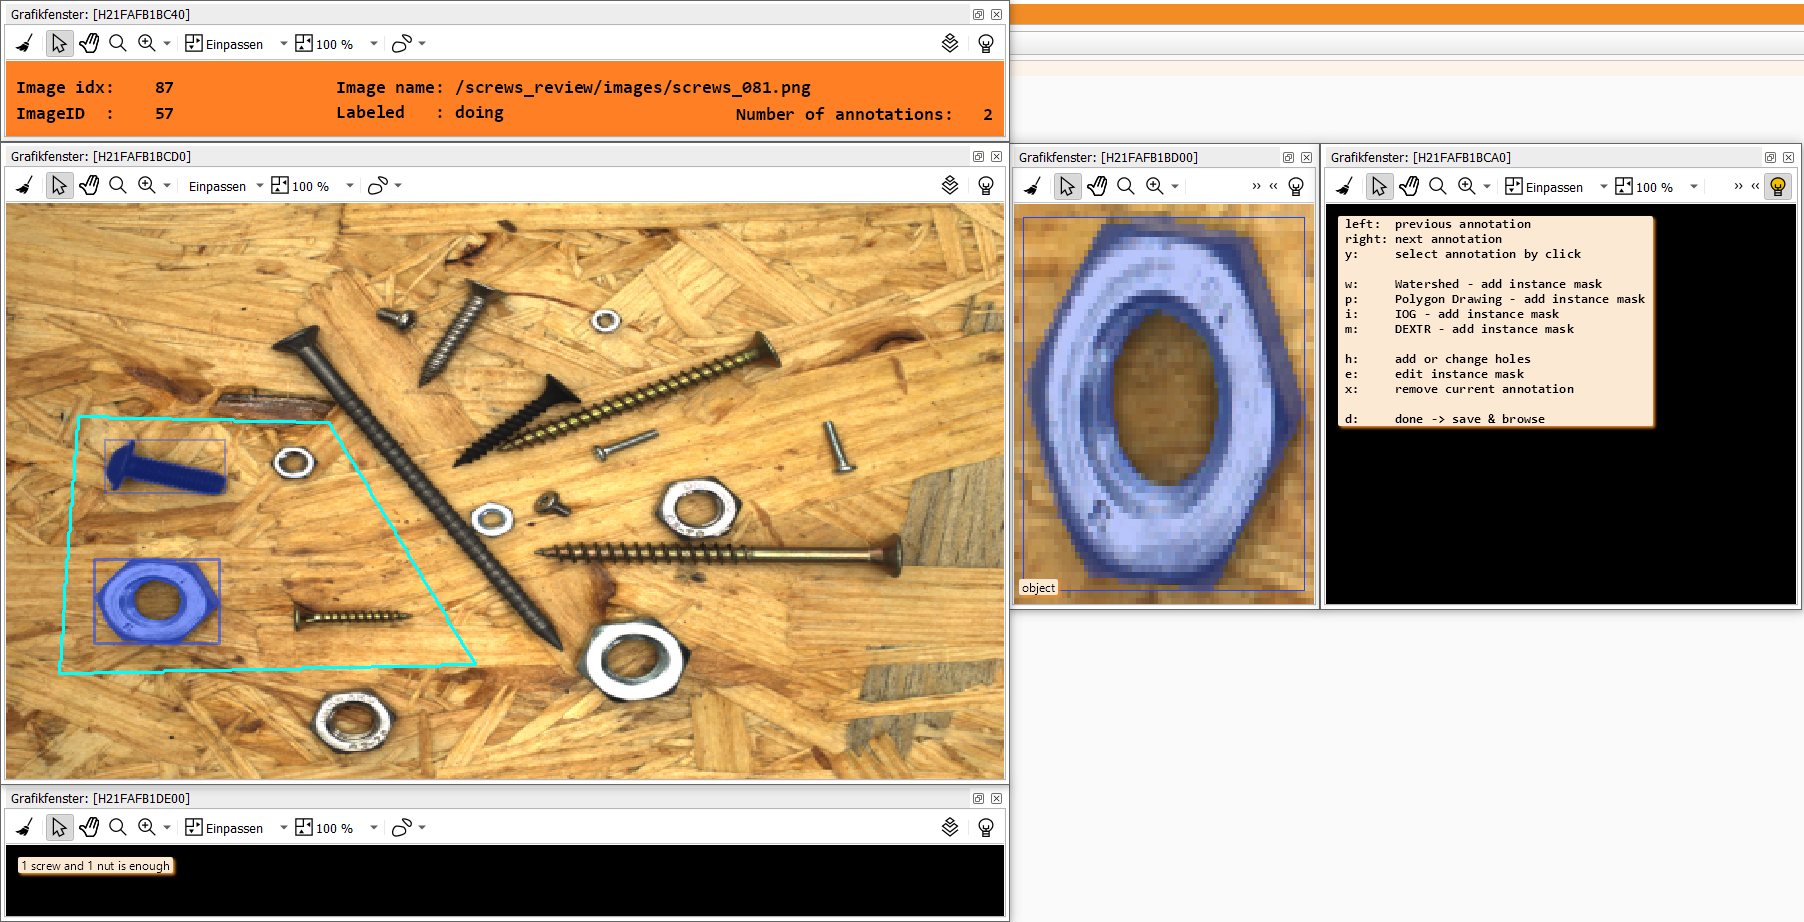
\includegraphics[width=\linewidth]{figures/chap45_labeltool_scrennshot.png}
	\caption[Screenshot of the user interface from the labeltool]{		
		Screenshot of the user interface from the labeltool implemented in HDevelop.
		The image origins from the MVTec Screws Dataset.
		It contains two annotation masks colored in blue and the label region as turquoise colored polygon.
		The smaller image window displays the currently selected annotation zoomed in.
		The window on the right, presents the user with the available options and the corresponding control key.
		On the bottom is a small window with a label instruction.
	}
	\label{fig:ch4:sec4:labeltool}
\end{figure}

